\documentclass[border=1pt]{standalone}
% Shared preamble for standalone figures in this directory.
% Compile with XeLaTeX from 讲义/figs, or via the figures target.
\usepackage{ctex}
\usepackage{amsmath}
\usepackage{amssymb}
\usepackage{bm}
\usepackage{mathtools}
\usepackage{tikz}
\renewcommand{\vec}[1]{\boldsymbol{#1}}
\newcommand{\cC}{\mathcal{C}}
\newcommand{\cD}{\mathcal{D}}
\newcommand{\R}{\mathbf{R}}
\usetikzlibrary{
    arrows.meta,
    calc,
    decorations.markings,
    angles,
    quotes,
    positioning,
    patterns,
    shapes.geometric
}

\begin{document}
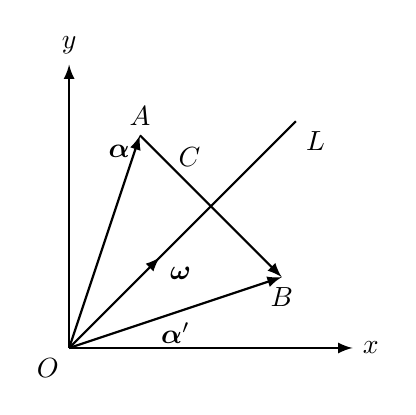
\begin{tikzpicture}[scale=1.8]
    \tikzset{>=latex, every path/.style={thick}, ->-/.style={
        decoration={markings, mark=at position .4 with {\arrow{>}}}, postaction={decorate}
    }}
    \draw[->] (0, 0) -- (0, 2) node[above] {$y$};
    \draw[->] (0, 0) -- (2, 0) node[right] {$x$};
    \draw (0,0) coordinate (O)
        (0.5, 1.5) coordinate (A)
        (1.5,0.5) coordinate (B);
    \draw node[above] at (A) {$A$}
        node[below left] at (A) {$\boldsymbol{\alpha}$}
        node[below] at (B) {$B$};
    \draw[->] (O) -- (A);
    \draw[->] (O) -- (B)
        node[pos=.5, below] {$\boldsymbol{\alpha}'$};
    \draw[->] (A) -- (B)
        node[pos=.35, above=3pt] {$C$};
    \draw[->-] (O) -- (1.6, 1.6)
        node[pos=.4, below right] {$\boldsymbol{\omega}$}
        node[below right] {$L$};
    \draw node[below left] at (O) {$O$};
\end{tikzpicture}

\end{document}
